%%% LaTeX Template
%%% This template can be used for both articles and reports.
%%%
%%% Copyright: http://www.howtotex.com/
%%% Date: February 2011

%%% Preamble
\documentclass[paper=a4, fontsize=12pt]{scrartcl}	% Article class of KOMA-script with 11pt font and a4 format

\usepackage[english]{babel}															% English language/hyphenation
\usepackage[protrusion=true,expansion=true]{microtype}				% Better typography
\usepackage{amsmath,amsfonts,amsthm}										% Math packages
\usepackage[pdftex]{graphicx}														% Enable pdflatex
%\usepackage{color,transparent}													% If you use color and/or transparency
\usepackage[hang, small,labelfont=bf,up,textfont=it,up]{caption}	% Custom captions under/above floats
\usepackage{epstopdf}																	% Converts .eps to .pdf
\usepackage{subfig}																		% Subfigures
\usepackage{booktabs}																	% Nicer tables
\usepackage[utf8]{inputenc} % We want UTF8
\usepackage{url}


%%% Advanced verbatim environment
\usepackage{verbatim}
\usepackage{fancyvrb}
\DefineShortVerb{\|}								% delimiter to display inline verbatim text


%%% Custom sectioning (sectsty package)
\usepackage{sectsty}								% Custom sectioning (see below)
\allsectionsfont{%									% Change font of al section commands
	\usefont{OT1}{bch}{b}{n}%					% bch-b-n: CharterBT-Bold font
%	\hspace{15pt}%									% Uncomment for indentation
	}

\sectionfont{%										% Change font of \section command
	\usefont{OT1}{bch}{b}{n}%					% bch-b-n: CharterBT-Bold font
	\sectionrule{0pt}{0pt}{-5pt}{0.8pt}%	% Horizontal rule below section
	}


%%% Custom headers/footers (fancyhdr package)
\usepackage{fancyhdr}
\pagestyle{fancyplain}
\fancyhead{}														% No page header
\fancyfoot[C]{\thepage}										% Pagenumbering at center of footer
\renewcommand{\headrulewidth}{0pt}				% Remove header underlines
\renewcommand{\footrulewidth}{0pt}				% Remove footer underlines
\setlength{\headheight}{13.6pt}

%%% Equation and float numbering
\numberwithin{equation}{section}															% Equationnumbering: section.eq#
\numberwithin{figure}{section}																% Figurenumbering: section.fig#
\numberwithin{table}{section}																% Tablenumbering: section.tab#


%%% Title	
\title{ \vspace{-1in} 	\usefont{OT1}{bch}{b}{n}
		\huge \strut Eksperter i Team  \strut \\
		\Large \bfseries \strut Konseptdokument \strut
}
\author{ 									\usefont{OT1}{bch}{m}{n}
        Forfattere etc\\		\usefont{OT1}{bch}{m}{n}
        Norges teknisk-naturvitenskapelige universitet\\ \usefont{OT1}{bch}{m}{n}
        Institutt for kunst- og medievitenskap\\
}
\date{}

%%% Begin document
\begin{document}
\maketitle
% Add the chapters
\section{Introduksjon}\label{sec:intro}
Dette avsnittet skal gi et kort overblikk over hvordan resten av
dokumentet er strukturert, hvilke spillmessige bakgrunner hver av
deltagerene i gruppen hadde, og hvilke mål som ble satt med tanke på å
utvikle et spillkonsept og en eventuell prototype.
\subsection{Struktur}
Dokumentet er i hovedsak strukturert i 4 hoveddeler:
\begin{enumerate}
	\item Introduksjon (Avsnitt~\ref{sec:intro})
	\item Konseptet (Avsnitt~\ref{sec:konsept})
	\item Utforming (Avsnitt~\ref{sec:design})
	\item Teknisk (Avsnitt~\ref{sec:teknisk})
\end{enumerate}
Konseptdelen skal gi en overordnet forståelse for hva spillet handler
om. Utformingdelen skal gi dypere innsikt i hvordan spillet er bygd opp,
og hvilke elementer det består av.
\subsection{Gruppemedlemmene}
Herunder vil den spillmessige bakgrunnen til hvert gruppemedlem bli
beskrevet.
\begin{description}
\item[Kjetil Mehl (23)] \hfill \\
Han begynte sin spillkarriere med en Nintendo 64\cite{n64} i 1999. Da
var det eventyr og rollespill (se Seksjon~\ref{sec:sjangre}) som Legend
of Zelda\cite{legendofzelda} og Banjo Kazooie\cite{banjokazooie} som
stod i fokus. Da datamaskinen kom i hus gikk spillfokuset  over på
konkurransespill som Counter-Strike og Warcraft. Han har i hovedsak vært
en Nintendo fanboy\cite{fanboy}, men har i de senere år utvidet
kolleksjonen til å omfatte Xbox.
\item[Ina Sander Pedersen (26)] \hfill \\
I 1996 oppdaget hun Rayman\cite{rayman} til PC og var fra den dag frelst for serien, men skiftet raskt konsoll til Playstation. For Ina har sjangeren plattform vært en klar favoritt gjennom årene og da hun senere fikk Gameboy Pocket\cite{gameboy} gikk tiden med til Donkey Kong Country 2\cite{DKC2}. Etterhvert som årene har gått har hun skiftet mellom Nintendo og Playstation, samt prøvd ut endel forskjellige sjangertyper, men Rayman og Donkey Kong seriene er og blir favoritter. 
\item[Christian Aleksander Lysne (22)] \hfill \\
Christian var 8 år da han fikk sin første Nintendo 64\cite{n64} , med spillene Super Mario 64\cite{mario64} og Mario Kart\cite{mariokart}. Senere gikk det i Legend of Zelda\cite{legendofzelda} og Super Smash Bros\cite{smash}. Tekken\cite{tekken} var også  populært i oppveksten. Warcraft 3\cite{wc3} og Diablo 2\cite{diablo2} tok etter hvert over, og spilles fortsatt i perioder.
\item[Andreas Røysland Aarnes (25)] \hfill \\
Som seksåring prøvde Andreas Super Mario World\cite{supermarioworld} på Super Nintendo\cite{supernintendo} for første gang, og det var ikke før i 2011, da remaken New Super Mario Bros. Wii\cite{newsupermario} kom til Nintendo Wii\cite{wii}, at han igjen ble tilfredstilt innen spillverdenen. I mellomtiden har han låst seg til strategispill-seriene Warcraft\cite{wc3}, Command \& Conquer\cite{cc} og Age of Empires\cite{aoe}. 
\end{description}
\subsection{Mål}
Det overordnede målet for gruppen var å lage et spillkonsept hvert
gruppemedlem følte eierskap til, og var konformt med den valgte
problemstillingen (se Seksjon~\ref{sec:problemstilling}). En prototype i
tillegg til dette ville bli en bonus i forhold til målet.
\subsection{Prosessen}
Dette avsnittet forteller hvordan konseptet ble til ved å gå fra en
problemstilling, til en idè og til slutt et konsept. Den første delen av
denne prosessen var ikke iterativ, ettersom gruppen i praksis gikk fra
en vagt definert problemstilling, til en idè, for så å redefinere ideen
for å bedre passe den valgte problemstillingen. Prosessen gikk deretter
fra idè til konsept.
\subsubsection{Fra problemstilling til idè}
Det ble brukt mye tid på å utforske forskjellige ideer som var
interessante. Gruppen følte seg ikke veldig bundet av den opphavlige
problemstillingen, og eksperimenterte derfor med forskjellige ideer.
Gitt problemstillingen i Avsnitt~\ref{sec:problemstillingen} var det
naturlig å tenke på et spill som var turbasert eller sanntidsspill med
flere spillere. Etter flere runder internt ble det enighet rundt
følgende idè.
\begin{description}
\item[Energispillet med flerspillermodus] \hfill\\
Spillere skal organisere hver sin lille by, hvor fokuset er å forhandle
med hverandre på grunnlag av hvilke energitype de forskjellige byene
velger å gå for. En by som for eksempel fokuserer på kull kan raskt få
mye resurser, men ville påvirke sitt eget miljø lokalt, og senere hele
miljøet globalt.
\end{description}
Etter tilbakemeldinger fra landsbylederen viste deg seg derimot at ideen
ikke samsvarte godt nok med problemstillinga som var valgt. Dette førte
til restrukturering av den opphavlige ideen, for å få mer fokus på
gjenbruk og resirkulering. Følgende elementer fra ideen ble tatt med
videre:
\begin{itemize}
	\item Flerspiller
	\item Hver spiller har en base
	\item Bruk av søppel som ressurser, istedenfor energi
	\item Lokale faktorer kan påvirke det globale miljøet
\end{itemize}
\subsubsection{Redefinering av ideen}
Den opphavlige ideen skle over på å bli et rent konkurransespill, med
mindre fokus sanking/utvinning av resurser. For å minske ressursfokuset
ble det bestemt at hver øy er en ``søppeløy'', og målet til spilleren er
å fjerne alt søppelet på sin øy.  Ressurser blir utvinnet ved å
resirkulere søppelet på øya. Ved å legge inn denne vrien ble ideen mer
konformt med problemstillingen. 

%Det ble gjort koblinger opp mot et spill lignende Advanced
%Wars\cite{advancewars} eller Wordfeud\cite{wordfeud} med fokus på
%miljøet.

\section{Problemstilling}\label{sec:problemstilling}
Dette avsnittet vil ta for seg den valgte problemstillingen, hva som lå
til grunn dette valget, og hvordan gruppen tenkte seg et konsept rundt
problemstillingen.
\subsection{Selve problemestillingen}
Den valgte problemstillingen er gjengitt nedenfor:
\begin{quotation}
\large\emph{``Hvordan kan en belyse nytten av resirkulering og redusert forbruk,
lokalt og globalt, gjennom flerspiller-dataspill
''}
\end{quotation}

\section{Prosessen}
Dette avsnittet forteller hvordan konseptet ble til ved å gå fra en
problemstilling, til en idè og til slutt et konsept. Den første delen av
denne prosessen var ikke iterativ, ettersom gruppen i praksis gikk fra
en vagt definert problemstilling, til en idè, for så å redefinere ideen
for å bedre passe den valgte problemstillingen. Prosessen gikk deretter
fra idè til konsept.
\subsection{Fra problemstilling til idè}
Det ble brukt mye tid på å utforske forskjellige ideer som var
interessante. Gruppen følte seg ikke veldig bundet av den opphavlige
problemstillingen, og eksperimenterte derfor med forskjellige ideer.
Gitt problemstillingen i Avsnitt~\ref{sec:problemstillingen} var det
naturlig å tenke på et spill som var turbasert eller sanntidsspill med
flere spillere. Etter flere runder internt ble det enighet rundt
følgende idè.
\begin{description}
\item[Energispillet med flerspillermodus] \hfill\\
Spillere skal organisere hver sin lille by, hvor fokuset er å forhandle
med hverandre på grunnlag av hvilke energitype de forskjellige byene
velger å gå for. En by som for eksempel fokuserer på kull kan raskt få
mye resurser, men ville påvirke sitt eget miljø lokalt, og senere hele
miljøet globalt.
\end{description}
Etter tilbakemeldinger fra landsbylederen viste deg seg derimot at ideen
ikke samsvarte godt nok med problemstillinga som var valgt. Dette førte
til restrukturering av den opphavlige ideen, for å få mer fokus på
gjenbruk og resirkulering. Følgende elementer fra ideen ble tatt med
videre:
\begin{itemize}
	\item Flerspiller
	\item Hver spiller har en base
	\item Bruk av søppel som ressurser, istedenfor energi
	\item Lokale faktorer kan påvirke det globale miljøet
\end{itemize}
\subsection{Redefinering av ideen}
Den opphavlige ideen skle over på å bli et rent konkurransespill, med
mindre fokus sanking/utvinning av resurser. For å minske ressursfokuset
ble det bestemt at hver øy er en ``søppeløy'', og målet til spilleren er
å fjerne alt søppelet på sin øy.  Ressurser blir utvinnet ved å
resirkulere søppelet på øya. Ved å legge inn denne vrien ble ideen mer
konformt med problemstillingen. 
\begin{description}
\item[Garbarge Alert] \hfill\\
Spillerene skal organisere hver sin lille søppelfylt øy. Målet er å
fortest mulig kvitte seg med søppelet på sin øy. Dette kan bli gjort ved
resirkulering, eller ved å sabotere for de andre spillerene ved å flytte
ditt søppel over til dem. Utifra aksjonene til de forskjellige
spillerene kan både lokale og globale katastrofer inntreffe. Spilleren
som først rydder sin øy, eller som står igjen til sist vinner spillet.
\end{description}
Utifra denne korte beskrivinga begynte vi å arbeide opp mot et konkret
konsept, som beskrevet i Avsnitt~\ref{sec:konsept}.
%Det ble gjort koblinger opp mot et spill lignende Advanced
%Wars\cite{advancewars} eller Wordfeud\cite{wordfeud} med fokus på
%miljøet.

\section{Ideen}

\section{Spilldynamikken}

\section{Sjangeren}\label{sec:sjangre}
Om spillsjangre og sånt.



%Før vi endte opp med sanntidsstrategisjangeren vurderte vi imidlertid en rekke andre mulige sjangre for realiseringen av konseptet. Spesielt eventyr- og rollespillsjangeren ble sterkt vurdert.

Under vil vi beskrive en rekke sjangre som ble vurdert for realiseringen av \emph{Garbage Alert}. Legg dog merke til at navnet ble til en tid etter at sjangeren var valgt.

\subsection{Eventyr}\label{sec:eventyr}
Den første sjangeren som ble vurdert som utgangspunkt for realisering av spillet var eventyrsjangeren. Denne sjangeren er definert ved at en direkte kontrollerer en protagonist i en interaktiv historie. Spilldynamikken består gjerne av det å overvinne ens omgivelser ved utforskning og oppgaveløsning\footnote{Rollings, Andrew; Ernest Adams (2006), Fundamentals of Game Design, Prentice Hall}.

Der finnes en hel rekke undersjangre under eventyrsjangeren. Av spesiell interesse har pek-og-klikk- og action-eventyrsjangrene vært.
	
	\subsubsection{Pek-og-klikk-eventyr}

	Her vil en styre protagonisten ved å peke hvor en vil gå, peke på objekter en vil interagere med og peke på andre mennesker en vil snakke med. Underveis samler en objekter som kan brukes andre steder i spillverden, enten direkte eller gjennom å kombinere gjenstander med hverandre for å skape nye gjenstander som gjør en  stand til å avansere i spillet.

	Populære spill i denne sjangeren er \emph{Lucas Arts'} \emph{Monkey Island}-serien og \emph{Funcoms} \emph{Den Lengste Reisen}.


	\subsubsection{Action adventure}

	Her styrer en tradisjonelt én figur som gradvis finner og samler utstyr som gjør en sterkere og mer motstandsdyktig mot miljø og fiender.


	Populære spill i denne sjangeren er \emph{Nintendos} \emph{The Legend of Zelda} og \emph{Supergiant Games'} \emph{Bastion}.


% \subsection{Rollespill}\label{sec:rollespill}
% RPG



\subsection{Strategi}\label{sec:strategispill}
Den andre sjangeren som ble vurdert for å realisere ideen om et resirkulering- og gjenbruksspill var strategisjangeren. Sentralt i denne sjangeren er ressursforvaltning, noe vi og følte kunne brukes for å realisere et godt konsept.

	\subsubsection{Turbasert strategi}

	Her deles hvert spill inn i \emph{runder}, hvor hver spiller har en egen \emph{tur} til å utføre sine handlinger.


	Den observante leser vil kunne legge merke til at dette ikke er ulikt tradisjonelle brettspill, noe som tilkjennegis ved at mange av de første digitale strategispill var konverteringer av tradisjonelle brettspill.

	Av populære turbaserte strategispill finner vi \emph{Firaxis'} \emph{Sid Meier's Civilization} og \emph{Intelligent Systems'} \emph{Advance Wars}. % TODO: Kilder?



	\subsubsection{Sanntidsstrategi}

	I motsetning til turbaserte strategispill vil ikke hver spiller ha sin egen tur til å utføre sine handlinger, men alle spillere vil utføre sine handlinger samtidig.

	Blant de mer sentrale elementer ved sanntidsstrategispill er konseptene om ressurshåndtering. De fleste spill i denne sjangeren lar det være opp til brukeren å passe på at man til enhver tid har adekvate ressurser til å gjøre den en ønsker og å benytte seg av de rasjonelt. Et annet element som ofte er til stede er stein-saks-papir-balansering av enheter, hvor enhet A kontrer enhet B, B kontrer enhet C og enhet C kontrer enhet A.

	Av populære sanntidsstrategispill finner vi \emph{StarCraft} og \emph{Command \& Conquer}.


\subsection{Vårt valg}
Helt i starten av prosessen som førte til Garbage Alert, startet vi med å diskutere ulike typer eventyr-tilnærminger. Det føltes svært naturlig at i et spill som skal omhandle resirkulering og gjenbruk å låne elementer fra den sjangeren som ofte benytter slike mekanismer. Folk ønsket dog mer fartsfull opplevelse, og diskusjoner om å implementere Zelda-aktige elementer i spillet ble diskutert.

Samtidig ble en alternativ idé utforsket, i kraft av at enkelte ønsket å inkorporere flerspiller og konkurranse som en motivasjonsfaktor. Her startet ideen med å skape et brettspill-inspirert spill. Denne ideen utviklet seg fra å være et svært komplisert turbasert spill til å bli stadig enklere, og stadig raskere, fram til det Garbage Alert til slutt skulle bli; et sanntidsstrategispill.


%!TEX root = report.tex
\section{Grafisk fremstilling}\label{sec:artwork}
Under vil den grafiske fremstillingen av \emph{Garbage Alert} bli beskrevet
sammen med valgene som har blitt gjort. Dette vil illustreres med
skjermskudd.

Den grafiske fremstillingen i spillet er ment å være leken og rettet mot
barn i alle aldre, og er sterkt inspirert av den klassiske spillserien
Advance Wars. Videre har det å holde ting oversiktlig og stort nok til å
trykkes på en berøringsskjerm vært noe vi har hatt spesielt i tankene
når grensesnittet har blitt utformet. Det er lagt mer vekt på
funksjonalitet, enn selve fremstillingen på denne delen av stadiet. Av
skjermskuddene ser en to forskjellige spillere som spiller mot
hverandre.

Som en ser av figur~\ref{fig:Oppgradering} kan spilleren på dette
tidspunktet kun oppgradere til plast. Dette er med andre ord i en tidlig
fase av spillet. Tilgjengelige ressurser er vist i bunnen av
skjermskuddet, og på dette tidspunktet kan miljøstasjonen kun gjenvinne
plast.

På figur~\ref{fig:Eksplosjon} har den blå spilleren angrepet den røde
spilleren, og man ser effekten av dette i eksplosjonen.

\begin{figure} [H]
\centering
\setlength\fboxsep{0.2pt}
\setlength\fboxrule{0.7pt}
\fbox{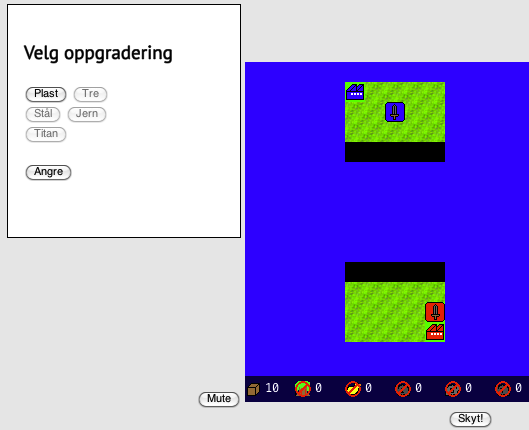
\includegraphics[width=\textwidth]{images/Oppgradering.png}}
\caption{Miljøstasjonen kan oppgraderes til å håndtere ulike typer avfallsgjenvinning.}
\label{fig:Oppgradering}
\end{figure}

\begin{figure}
\centering\setlength\fboxsep{0.2pt}
\setlength\fboxrule{0.7pt}
\fbox{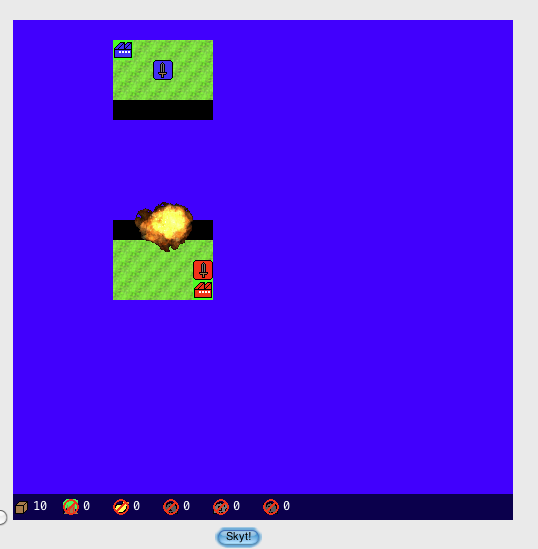
\includegraphics[scale=0.5]{images/Eksplosjon.png}}
\caption{Ved et angrep på en annen spiller vil et projektil avfyres og eksplodere på motspillerens eventuelle forsvarsstruktur.}
\label{fig:Eksplosjon}
\end{figure}

\begin{figure}
\centering
\setlength\fboxsep{0.2pt}
\setlength\fboxrule{0.7pt}
\fbox{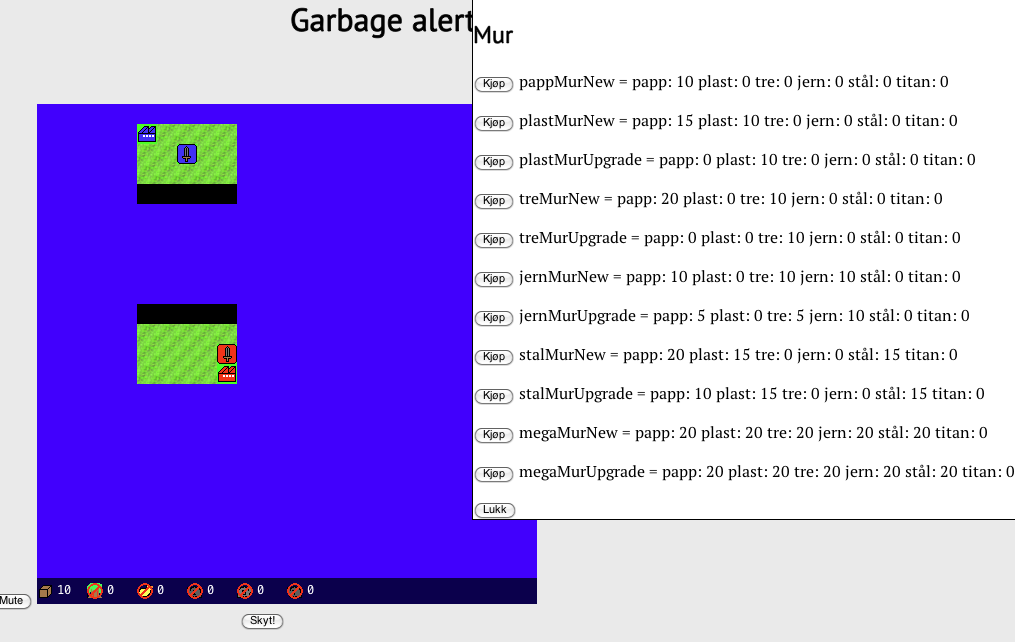
\includegraphics[width=\textwidth]{images/OppgradereMur.png}}
\caption{Spillerens forsvarsstruktur kan oppgraderes til å håndtere sterkere skyts fra motspilleren, avhengig av tilgjengelige ressurser.}
\label{fig:OppgradereMur}
\end{figure}

\begin{figure}
\centering
\setlength\fboxsep{0.2pt}
\setlength\fboxrule{0.7pt}
\fbox{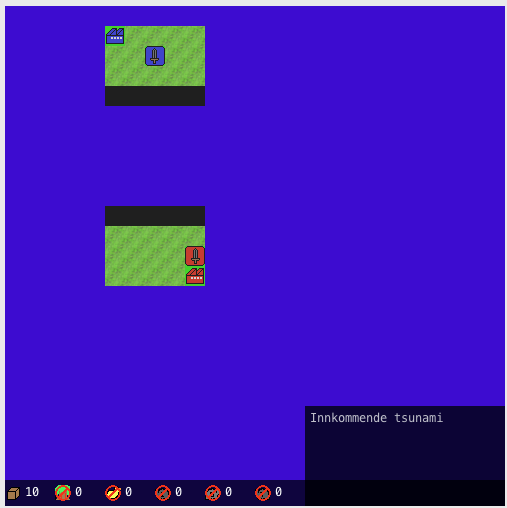
\includegraphics[scale=0.5]{images/Tsunami.png}}
\caption{Globale geohasarder kan oppstå som følge av mye global forsøpling, som for eksempel en tsunami.}
\label{fig:Tsunami}
\end{figure}

\begin{figure} 
\centering
\setlength\fboxsep{0.2pt}
\setlength\fboxrule{0.7pt}
\fbox{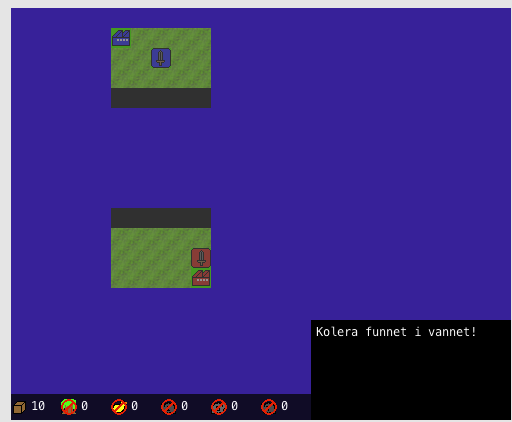
\includegraphics[scale=0.7]{images/Kolera.png}}
\caption{Lokale biohasarder kan oppstå som følge av mye lokal forurensning. Her er et sykdomsutbrudd.}
\label{fig:Kolera}
\end{figure}

\begin{figure} [H]
\centering
\setlength\fboxsep{0.2pt}
\setlength\fboxrule{0.7pt}
\fbox{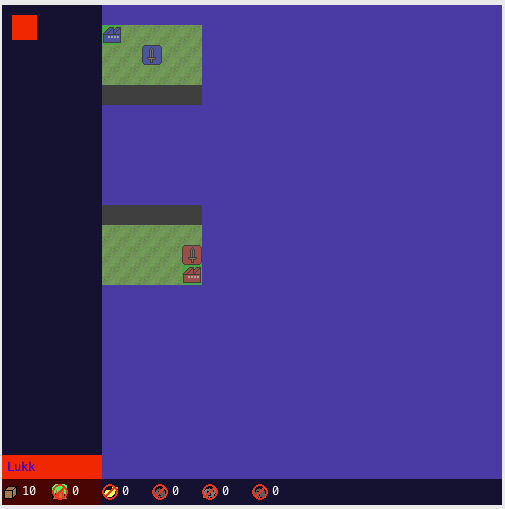
\includegraphics{images/OppgradereEnv.png}}
\caption{Miljøstasjonens effektivitet kan oppgraderes slik at den gjenvinner mer materialer fra hver avfallsenhet.}
\label{fig:OppgradereEnv}
\end{figure}

På figur~\ref{fig:OppgradereEnv} har den røde spilleren åpnet
oppgraderingsmenyen sin. Her har han mulighet til å oppgradere
effektiviteten av miljøstasjonen sin.

Legg merke til at disse skjermskuddene er tatt av en veldig tidlig
prototype som har hatt fokus på å implementere så mye av den tenkte
funksjonaliteten som mulig, heller enn å etablere et konsistent grafisk
uttrykk. Det var ønskelig å benytte så mye som mulig av den kode og
grafikk som ble til i vår tidlige prototype videre i den mer avanserte
prototypen\footnote{Noen vil kanskje si at dette ble gjort i tråd med
landsbyens filosofi om gjenbruk og gjenvinning.}. Mot en sluttfase vil
det være naturlig å erstatte eksempelgrafikken med noe grafikk som er
mer polert.


\begin{thebibliography}{9} %antall ref?
\bibitem{n64}
	Nintendo 64 - \url{http://www.old-computers.com/museum/computer.asp?c=1242&st=2}
\end{thebibliography}

\end{document}
